% template.tex, dated April 5 2013
% This is a template file for Annual Reviews 1 column Journals
%
% Compilation using ar-1col.cls' - version 1.0, Aptara Inc.
% (c) 2013 AR
%
% Steps to compile: latex latex latex
%
% For tracking purposes => this is v1.0 - Apr. 2013

\documentclass[a4paper]{ar-1col}


\usepackage[comma]{natbib,amssymb}

\setcounter{secnumdepth}{4}

% Metadata Information
\jname{Annu. Rev. Astron. Astrophys.}
\jvol{58}
\jyear{2020}
\doi{10.1146/((please add article doi))}

%\bibliographystyle{ar-style2.bst}
\bibliographystyle{aasjournal.bst}

% Document starts
\begin{document}

% Page header
\markboth{Andrews}{Disk Structures}

% Title
\title{Observing the Structures of Protoplanetary Disks}


%Authors, affiliations address.
\author{Sean M. Andrews
\affil{Center for Astrophysics \textbar\ Harvard \& Smithsonian \\ Cambridge, Massachusetts, USA 02138; email: sandrews@cfa.harvard.edu}}

%Abstract
\begin{abstract}
Debris disks are tenuous, dust-dominated disks commonly observed around
stars over a wide range of ages. Those around main sequence stars are analogous
to the Solar System’s Kuiper Belt and zodiacal light. The dust in debris
disks is believed to be continuously regenerated, originating primarily with
collisions of planetesimals. Observations of debris disks provide insight into
the evolution of planetary systems; and the composition of dust, comets,
and planetesimals outside the Solar System; as well as placing constraints
on the orbital architecture and potentially the masses of exoplanets that are
not otherwise detectable. This review highlights recent advances in multiwavelength,
high-resolution scattered light and thermal imaging that have
revealed a complex and intricate diversity of structures in debris disks and
discusses how modeling methods are evolving with the breadth and depth of
the available observations. Two rapidly advancing subfields highlighted in
this review include observations of atomic and molecular gas around main
sequence stars and variations in emission from debris disks on very short
(days to years) timescales, providing evidence of non-steady-state collisional
evolution particularly in young debris disks.
\begin{itemize}
\item First finding.
\item Second finding.
\item Third finding.
\end{itemize}
\end{abstract}

%Keywords, etc.
\begin{keywords}
keywords, separated by comma, no full stop, lowercase
\end{keywords}
\maketitle

%Table of Contents
\tableofcontents


\section{INTRODUCTION} \label{sec:intro}

\subsection{Motivation} \label{sec:motivation}

The formation and early evolution of a star and its planets are fundamentally governed by their relationships with a circumstellar disk.  The telltale signatures of the foundational interactions between disk, star, and planets are imprinted on the disk structure -- the detailed spatial distribution and physical conditions of the disk material.  Measurements of disk structures, complemented with theoretical simulations, can be used to figure out how the key physical mechanisms associated with star and planet formation operate. 

Star formation begins with the gravitational collapse of an over-density (core) in a molecular cloud.  Rotation of that core implies that material from its outer regions, with higher angular momentum, is channeled onto a flattened disk that orbits a central protostar, rather than directly onto the star itself \citep{cassen81,terebey84}.  In that sense, disks are a simple consequence of angular momentum conservation.  Measurements of young disk structures, still embedded in their natal core material (envelope), reveal much about the star formation process: their sizes help distinguish the roles that magnetic fields have in regulating core collapse; their masses constrain the typical protostellar accretion rates; and their density distributions encode the mechanics of angular momentum transfer and accretion that ultimately determine the stellar mass.  

Disks are also the birthplaces of planetary systems.  The prevalence, formation modes, masses, orbital architectures, and compositions of planets depend intimately on the physical conditions in the disk at their formation sites, the evolution of that disk structure (locally and globally), and the planetary migration driven by dynamical interactions with the disk material.  Measurements of the disk mass and its spatial distribution offer crucial boundary conditions for models of planet formation.  Combined with the demographic properties observed in the mature exoplanet population, that information can help develop and refine a predictive formation theory, despite the considerable complexity of the associated physical processes \citep[e.g.,][]{ida04,alibert05}.



\subsection{Observational Primer} \label{sec:primer}

In many ways, disk structures offer profound insights on how the properties of stars and planetary systems are shaped by their origins.  This review is focused on the recent landscape of observational constraints on disk structures: how relevant measurements are made, what they suggest about disk properties, and how those properties are connected to star and planet formation.  The key measurements of disk structures require high angular resolution data, as the typical disk in a nearby star-forming region subtends only $\sim$1$^{\prime\prime}$ on the sky.  Most of any given disk is relatively cool enough (temperatures $<$100 K) that it emits most efficiently in the millimeter-wave part of the spectrum (hereafter mm, meaning $\lambda \approx 0.5$--5 mm).  Coupling these small angular sizes and cool temperatures, considerable emphasis in this review will be placed on radio interferometry as an essential tool.  Indeed, dramatic progress over the past decade has largely been driven by the commissioning of the transformational Atacama Large Millimeter/submillimeter Array (ALMA) facility.
\begin{marginnote}[]
\entry{sub-mm}{$\lambda \approx 0.1$--0.5 mm, $\nu \approx 0.6$--3 THz.}
\entry{mm}{$\lambda \approx 0.5$--5 mm, $\nu \approx 60$--600 GHz.}
\entry{cm}{$\lambda \approx 5$--50 mm, $\nu \approx 6$--60 GHz.}
\end{marginnote}

Three categories of observational tracer are useful for studying disk structures: scattered light, thermal continuum emission, and (primarily molecular) spectral line emission.  The first two are sensitive to the physical conditions and distribution of solids, and the third is used to measure the properties of the gas.  Each observational probe is sensitive to different materials and physical conditions, ensuring considerable diversity in the disk appearance when viewed in different tracers.  An illustrative example is shown in {\bf Figure \ref{fig:ims}}. 


\subsubsection{Scattered Light}
Small ($\mu$m-sized) dust grains suspended in the disk atmosphere can reflect the optical and infrared radiation emitted by the the central host star.  This scattered light is especially sensitive to the vertical distribution of the dust, and how it changes with radius \citep[e.g.,][]{debes13,stolker16,garufi17}.  Spectral and polarization variations in the scattered light morphology can constrain the albedo and phase function of the scatterers, which are set by the size, shape, and composition of the grains \citep{debes08,min12,min16}.  Aside from uniquely probing the dust disk surface geometry, the key advantage of this tracer is resolution: adaptive optics systems operating at the diffraction limit on 8--10 m telescopes measure features at 30--50 mas scales ($\sim$5 au).  The important challenges are contrast with the host stars, which prevent measurements in the innermost disk ($\lesssim 10$ au), and sensitivity at large radii, due to the $1/r^2$ dilution of the stellar radiation field.  The latter issue has limited the sample of resolved scattered light measurements, and biased it toward disks with brighter (earlier type) hosts.    

%The continuum and line emission are thermal radiative processes, so the kind of information about the disk structure available from a given tracer depends on its optical depth, $\tau_\nu$.  If the tracer emission is optically thin ($\tau_\nu \ll 1$), the intensity scales roughly with the product $I_\nu \propto X B_\nu(T) N$, where $B_\nu(T)$ is the Planck function at the local temperature, $N$ is column density, and $X$ is a (potentially complicated) conversion factor that quantifies how much emission is produced per unit mass for that tracer species.  With some information on $X$, $T$, and the disk geometry, a measurement of $I_\nu$ offers a density constraint.  If the emission is optically thick ($\tau_\nu \gtrsim 1$), the intensity scales with the temperature at the effective photosphere of the tracer, $I_\nu \propto B_\nu(T)$.  In this case, only lower bounds on the densities of the tracer species are available, and the emission can be affected by scattering.          

\subsubsection{Continuum Emission}
Disk solids also emit their own thermal continuum radiation that spans at least four decades in wavelength (from 1 $\mu$m to 1 cm).  Most of that emission is optically thick, and therefore a diagnostic of the temperature structure in the disk \citep[e.g., see][]{andrews15}.  Lower optical depths ($\tau_\nu$) are available at longer wavelengths, with the transition to optically thin traditionally expected in the sub-mm \citep{beckwith90}.  In the optically thin limit ($\tau_\nu \ll 1$), the continuum intensities scale with the product $I_\nu \propto \kappa_\nu B_\nu(T) \Sigma_s$, where $\kappa_\nu$ is the opacity (absorption cross section per unit mass), $B_\nu(T)$ the Planck function at the local temperature $T$, and $\Sigma_s$ the surface density of solids.  The mm continuum spectrum has a roughly power-law shape, $I_\nu \propto \nu^{\alpha_{\rm mm}}$, with the spectral index set by the sum of contributions from the Planck function ($B_\nu \propto \nu^{\alpha_{\rm Pl}}$, where $\alpha_{\rm Pl} \approx 1.7$--2.0 for $T > 15$ K) and the opacity spectrum ($\kappa_\nu \propto \nu^\beta$), $\alpha_{\rm mm} \approx \alpha_{\rm Pl} + \beta$ \citep{beckwith91,ricci10a,ricci10b}.  The opacity index, $\beta$, depends on the sizes, shapes, and compositions of the solids \citep{miyake93,dalessio01,draine06}.  

In principle, resolved measurements of the mm continuum provide an ideal opportunity to constrain the mass distribution (and particle properties) of the disk solids.  This tracer is also relatively easy to observe at high resolution, down to 10--20 mas scales ($\sim$2 au; and no contrast issues with the host), thanks to the large bandwidths of modern interferometers.  This means measurements are plentiful: much of the collective knowledge of resolved disk structures is based on mm continuum observations.  There are two key sources of ambiguity in interpreting these data.  First, some of the emission could be optically thick, perhaps preferentially in the inner disk \citep[see][]{beckwith90,aw05}.  In that case, the intensities saturate to $B_\nu(T)$ and the spectral index reverts to $\alpha_{\rm Pl}$.  Self-scattering could even diminish the intensities below $B_\nu(T)$ and permit $\alpha_{\rm mm}$ to vary in the range 1.5--2.5, depending on the frequency dependence of the albedo \citep{zhu19,liu19}.

\subsubsection{Spectral Line Emission}




\subsection{Statement of Scope} \label{sec:scope}

This review covers four broad (and in most respects inter-related) topics that currently occupy much of the effort in the disk community: the impetus and techniques for measuring key properties of disk structures, like masses and density distributions (Section \ref{sec:structure}); the constraints on evolutionary and environmental dependencies based on demographics studies (Section \ref{sec:demographics}); the evidence for (and problems with) the growth and migration of disk solids (Section \ref{sec:solids}); and the properties and roles of small-scale {\it substructures} in shaping observables and facilitating planet formation (Section \ref{sec:substructures}).  It concludes with a summary (Section \ref{sec:summary}) and a discussion of some potentially fruitful avenues for future work (Section \ref{sec:future}).  




\section{KEY\ STRUCTURE\ PROPERTIES} \label{sec:structure}

The spatial distribution of mass -- the density structure -- is without question the fundamental property of interest for disks.  The over-arching conceptual design of the field presumes that disk evolution is basically deterministic, such that a collection of ``snapshots" of disk density distributions that span an appropriate range of environmental and evolutionary states could be used to work out the mechanics of key physical processes and thereby refine a predictive model of how disks regulate star and planet formation.  This section of the review is focused on the underlying motivations, observational tracers, and lingering ambiguities associated with attempts to measure the mass distributions in disks.  Since the density structure is intrinsically tied to the thermal and dynamical state of the disk, constraints on temperatures (Section \ref{sec:temp}) and kinematics (Section \ref{sec:turb}) are also summarized.        

\begin{textbox}[h]\section{Notation, Conventions, and Nomenclature}
To set the practical framework for interpreting the results in this field, some discussion of standards and terminology is helpful.  The common characterization of the density structure in disks essentially condenses to a one-dimensional description through the radial surface density profil  e, $\Sigma$, defined such that the mass $M = 2\pi \int \Sigma \, r \, dr$.  This is not intended to diminish the azimuthal or vertical dimensions (with coordinates $\varphi$ and $z$, respectively), but rather reflects both a convenient simplification and the fact that disks are by their nature geometrically thin.  Because of their different physical and observable behaviors, it is also useful to differentiate the disk contents into two broad categories, solids and gas; their density profiles are related by the (vertically averaged) solids-to-gas ratio, $\zeta = \Sigma_s / \Sigma_g$.  The goals of this section are to motivate the physical interest in $\Sigma_s$ and $\Sigma_g$, establish the related observable properties, summarize the state of measurements, review some important limitations, and outline the links to the thermal and dynamical structures of disks.  
\end{textbox}



\subsection{Masses} \label{sec:mass}

Most of the emphasis in the field is on the integrated quantity, disk masses, rather than their density distributions.  That is mostly a practical limitation, but many of the key techniques and issues can be illustrated well from this coarser perspective.  The primary interest here is that measurements of disk masses offer elementary constraints on the contents of planetary systems.  Summing the terrestrial planet and giant planet core masses offers a conservative lower bound on the solid mass of the Solar Nebula disk ($M_s > 45 M_\oplus$; \citealt{weidenschilling77}) or its exoplanet counterparts \citep[e.g.,][]{chiang13}.  Extrapolations of the current planetary atmosphere contents to the primordial H,He-rich gas expected in disks \citep[e.g.,][]{kusaka70} enable an analogous limit for the gas masses ($M_g > 0.01 M_\odot$; e.g., \citealt{hayashi81}).  The current census of exoplanets finds an abundance of worlds orbiting other stars \citep{howard10,dressing13}, but the efficiency of the metamorphosis of disk material into planetary systems is unclear without a comparison of the mass reservoirs in the parent and descendent populations.          


\subsubsection{Observational Tracers}
Disk solids are a minor contributor to the total mass ($\sim$1\%), but the crucial roles they play in all aspects of disk evolution and planet formation justify special attention to their mass reservoir, $M_s$.  Solids emit a broadband thermal continuum spectrum that depends on their temperature and microphysical properties (composition, internal structure, size).  Assuming reasonable properties for the solids and disk physical conditions, optical depths have traditionally been expected to be low enough at microwave wavelengths that the continuum luminosity is proportional to $M_s$ \citep{beckwith90}.  
\begin{marginnote}[]
\entry{microwave}{Generic term adopted here to refer to wavelengths from a few hundred $\mu$m to a few cm.}
\end{marginnote}

Of course, the continuum spectrum emitted by solids in a typical disk spans at least four decades in wavelength ($\sim$1 $\mu$m to 1 cm).  But most of it is optically thick, and therefore more a diagnostic of the thermal structure than the mass.  High resolution infrared imaging can also trace scattered starlight from the small solids lofted high above the disk midplane, but again such measurements are insensitive to the mass.  While these alternate tracers are unquestionably informative in other contexts, the comparatively bright microwave continuum and its unique access to $M_s$ make it an especially valuable probe.            

Most of the mass in a disk is H$_2$ gas.  However, H$_2$ lacks a permanent dipole moment and is therefore essentially `dark': there is no {\it direct} probe of the dominant gas reservoir.  Constraints on gas masses in disks ($M_g$) must instead be derived from the spectral line emission of rarer molecule species.  The optimal tracers are optically thin emission lines from molecules that have a reasonably well-understood abundance relative to H$_2$.  In such a case, the emission line luminosity can be converted into a measurement of $M_g$.

In the literature, two tracer molecule options have been considered for $M_g$ constraints: HD (the primary isotopologue of H$_2$) and CO.  The advantage of HD is the simplicity of its associated chemical network, meaning the HD/H$_2$ abundance ratio is known well \citep{bergin13,mcclure16,trapman17}.  But with a ground state transition in the far-infrared (112 $\mu$m), HD measurements are scarce (and currently inaccessible).  CO is a popular alternative, but the rotational lines from the primary isotopologue are very optically thick \citep{beckwith93}.  Therefore, gas mass estimates rely on line luminosity measurements of rarer isotopologues, usually $^{13}$CO and C$^{18}$O together \citep{williamsbest14}.  The advantages of CO tracers are practical, since these lines are (relatively) bright and accessible (with a sequence of transitions throughout the microwave spectrum), but their abundances are more uncertain.  For reference, the utility of a suite of (less favorable) alternative tracers for $M_g$ measurements were explored by \citet{molyarova17}.


\subsubsection{Overview of Mass Measurements}
The advent of bolometer detectors on single-dish microwave telescopes motivated a series of continuum photometry surveys designed to measure $M_s$ for hundreds of disks starting 30 years ago \citep{weintraub89,beckwith90,andre94,osterloh95,aw05,aw07b}, and continuing today with more sensitive interferometers \citep[e.g.,][]{andrews13,ansdell16,cieza19}.  The microwave continuum luminosities (hereafter $L_{\rm mm}$) from these surveys span at least three orders of magnitude.  Though this composite $L_{\rm mm}$ distribution is clearly influenced by observational and physical selection effects (see Section \ref{sec:demographics}), it helps provide some rough guidance on $M_s$ values.  For some fiducial assumptions for the disk-averaged temperature ($\langle T \rangle \approx 20$ K, based on crude models of infrared emission; \citealt{aw05}) and opacity ($\langle \kappa_\nu \rangle \approx 2.3$ cm$^2$ g $^{-1}$ at $\lambda = 1.3$ mm, as asserted by \citealt{beckwith90}), these luminosities imply a range $M_s \approx 1$--1000 $M_\oplus$.
% additional photometry surveys: 
% single-dish = reipurth93, henning93, jensen94, jensen96, nurnberger98, cieza15, ansdell15; 
% interferometry = williams05, mann09, mann10, mann14, mann15, harris12, akeson14, akeson19, carpenter14, pascucci16, vanderplas16, barenfeld17, ansdell17, law17, eisner06, eisner08, eisner16, cox17, eisner18, ward-duong18, ruiz-rodriguez18

There are many fewer available estimates of $M_g$ in disks, owing to the intrinsically more challenging observations of the emission line tracers.  The ground state HD emission line was detected from only three disks, suggesting $M_g \ge 0.01 M_\odot$ based on detailed models of their thermal structures \citep{bergin13,mcclure16}.  Larger samples of CO isotopologue emission line luminosities typically infer considerably lower values, $M_g < 0.001 M_\odot$ \citep[and detection rates are relatively low; e.g.,][]{ansdell16,long17}, when referenced to an extensive grid of model structures that assumes the CO/H$_2$ abundance in disks is comparable to the interstellar medium \citep{williamsbest14}.     


\subsubsection{Caveats and Ambiguities}
There are large uncertainties in any inference of $M_s$ from microwave continuum data, for two primary reasons.  First, the assertion that the emission is optically thin is unlikely to be valid at all disk locations.  Once optical depths are high, the emission saturates and mass is hidden ($M_s$ is under-estimated).  The significance of this effect depends on the surface area of the thick emission, which will be revisited in various contexts throughout this review.  Second, even in the $\tau_\nu \ll 1$ limit, the continuum luminosity scales with the product of the temperature, opacity, and mass.  The uncertainty in $T$ will be addressed in Section \ref{sec:temp}.  There is considerable ambiguity in $M_s$ estimates due solely to our relative ignorance of the microphysical particle properties that set $\kappa_\nu$, including their mineralogical (and ice) compositions \citep{pollack94}, sizes \citep{miyake93}, and internal structure (porosity; \citealt{henning96}).  

%Information about the compositions of disk solids can be accessed through spectral features in the infrared, particularly from silicates \citep{kessler-silacci06,bouwman08,sargent09b} and common ices \citep{oberg08,bottinelli10,mcclure15}.  Various carbonaceous materials are also expected to be primary constituents \citep{zubko96,jaeger98}.  The implied compositions are commensurate with {\it in situ} measurements of dust particles, meteorites, and larger ``primordial" bodies in the Solar System \citep[e.g.,][]{clayton04,mumma11}.  In that sense, the composition-related ambiguities in $\kappa_\nu$ are probably less associated with the mineralogy and more on lingering uncertainties in the corresponding dielectric properties and how those are combined for realistic composites \citep[e.g.,][]{min16,demyk17}.  

Because the particle properties encoded in $\kappa_\nu$ are so fundamentally important for interpreting observations, this latter issue is worth elaboration.  The sizes and morphologies of the emitting particles have the most pronounced effects on the behavior of $\kappa_\nu$.  Size distributions are often approximated as power-laws, $n(a) \propto a^{-q}$ for size (radius) $a \in [a_{\rm min}, a_{\rm max}]$, with indices comparable to the expectation for a self-similar collisional cascade ($q \approx 3.5$; \citealt{dohnanyi69,tanaka96}) or more top-heavy variants ($q \approx 2.5$; e.g., \citealt{birnstiel11}).  The particle morphologies are characterized by their porosities, usually parameterized with a volume filling factor $f_s$ ($\sim$1 for compact particles, but can be as low as $\sim$10$^{-4}$ in aggregates; \citealt{kataoka13}).  The microwave opacity spectrum is roughly a power-law, $\kappa_\nu \approx \kappa_0 (\nu/\nu_0)^\beta$, where $\kappa_0$ and $\beta$ both depend on \{$q$, $a_{\rm max}$, $f_s$\}.  

For reference, Figure \ref{fig:opac} illustrates how opacity properties generally respond to particle properties, for some representative model variations (see \citealt{cuzzi14}, \citealt{woitke16}, or \citealt{dsharp5} for more detailed explorations of the parameter-space). When $a_{\rm max} \ll \lambda$, $\kappa_0$ is roughly independent of the size cut-off and $\beta$ is high ($\sim$1.7, as for the small dust grains in the interstellar medium; \citealt{finkbeiner99}).  When $a_{\rm max} \gg \lambda$, $\kappa_0$ decreases with $a_{\rm max}$ at a rate depending on $q$ (lower $q$ means a steeper fall-off; e.g., \citealt{ricci10a}) and $\beta$ is lower (scaling roughly with $q$; \citealt{draine06}).  When $a_{\rm max} \sim \lambda$, resonances drive up both $\kappa_0$ and $\beta$.  Porosity dampens those resonant amplifications.  Specifically, $\kappa_\nu$ varies with the product $a_{\rm max} f_s$, such that porous particles have a lower $\kappa_0$ and higher $\beta$ than compact particles with the same size distribution \citep{kataoka14}.  

\begin{figure}[t]
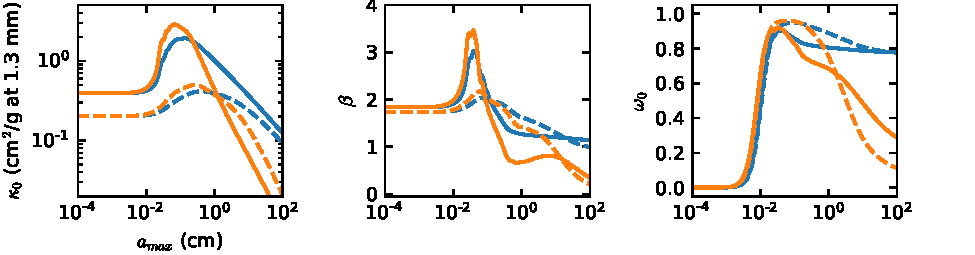
\includegraphics[width=\textwidth]{opac_pars.pdf}
\caption{kappa0, beta, albedo as fn of amax (different q, phi, composition, mixing rule, DDA v Mie)}
\label{fig:opac}
\end{figure}

While continuum luminosities cannot constrain $\kappa_0$, information about the particle properties are accessible from the {\it shape} of an optically thin microwave spectrum, which varies like $L_\nu \propto \kappa_\nu B_\nu(T) \propto \nu^{\alpha_{\rm mm}}$.  The spectral index (i.e., the ``color") tracks the opacity index, $\alpha_{\rm mm} \approx \alpha_{\rm Pl} + \beta$, where $\alpha_{\rm Pl} \approx 1.7$--2.0 approximates the shape of $B_\nu(T)$ for disk-averaged temperatures $>$15 K.  Multiwavelength photometry surveys find $\alpha_{\rm mm} \approx 2$--3 \citep{beckwith91,mannings94,ricci10a,ricci10b,ricci12}, implying a disk-averaged $\beta \le 1$ and $a_{\rm max} \ge 1$ mm.  There is a sort of apocryphal notion that continuum emission traces particles with sizes up to $a_{\rm max} \sim \lambda$.  But a more accurate statement is that the emission is most {\it efficient} with this criterion since it corresponds to the peak $\kappa_0$ (giving the most emission per mass), but even much larger particles still contribute.  Therein lies the key ambiguity: the opacity can decrease (by orders of magnitude) if larger solids are present (see Fig.~\ref{fig:opac}), and the ambiguities of interpreting $\beta$ constraints permit such a possibility.  Note that the fiducial opacities adopted in the literature ($\sim$1--3 cm$^2$ g$^{-1}$ at $\lambda = 1.3$ mm) are effectively upper bounds on $\kappa_\nu$ (see Fig.~\ref{fig:opac}), reflecting the fact that $L_{\rm mm}$ measurements are really yielding lower limits on $M_s$. 

Unresolved spectral index measurements naturally gloss over some important complexities.  The particle properties, and thereby the opacities, are expected to vary spatially in disks.  The (presumably inter-dependent) morphologies of those variations make it difficult to determine the impact of $\kappa_\nu$ changes on inferences of $M_s$ without spatially resolved measurements of $\alpha_{\rm mm}$.  Moreover, an unknown fraction of the continuum emission can be optically thick, where $\alpha_{\rm mm} \approx 1.5$--2.5 depending on $T$ (or $\alpha_{\rm Pl}$) and the spectral dependence of the albedo \citep{zhu19,liu19}.  This would diminish unresolved (disk-averaged) estimates of $\beta$, again limiting an assessment of the $M_s$ uncertainty due to the opacities.

Shifting attention to the gas mass, there are direct analogues of these same ambiguities.  First, there is also the concern that the optically thin approximation is at least partially invalid, particularly for the HD and $^{13}$CO lines, implying again that mass may be hidden ($M_g$ is under-estimated).  As with the microwave continuum, the emission from an optically thin spectral line traces the produce of temperature and column density (i.e., mass).  The key difference is that the line emission originates from a more two-dimensional geometry (radial and vertical), which can potentially incorporate pronounced temperature gradients that are directly related to the distribution of the tracer abundances.  This is especially significant for $M_g$ estimates from the HD ground state line, which by a quirk of its excitation physics has an exponential $T$ dependence \citep{bergin13}.  In any case, a good model or measurement of $T(r, z)$ is required for a robust estimate of $M_g$ (see Section \ref{sec:temp}).    

The key ambiguities in $M_g$ measurements from optically thin emission lines come from the uncertain chemical abundances of the tracer molecules relative to H$_2$.  For HD, the associated chemical network is simple enough that the gas phase abundance should be fairly robust; the open questions are related to the unaccounted contribution of enhanced D fractionation in ices or hydrocarbons that could lead to an under-estimate of HD/H$_2$ (and therefore $M_g$).  The situation with CO is more complicated.  Presuming the interstellar CO/H$_2$ abundance ratio and isotopic fractionation \citep{frerking82}, the observed CO isotopologue luminosities from disks suggest surprisingly low $M_g$ values (by a factor of $\sim$5--10; \citealt{williamsbest14}) relative to other gas tracers in the same disks \citep{chapillon10,favre13,kama16a} or estimates of $M_s$ and presumed interstellar solids-to-gas ratios ($\zeta \approx 0.01$; \citealt{kastner97,dutrey03,ansdell16,long17}).  This apparent anomaly can be reconciled by invoking a higher solids-to-gas ratio ($\zeta \ge 0.1$) or modifying the assumed abundances.  The right direction and amplitude of abundance changes are expected from various chemical processes, including adsorption onto solids (``freezeout"; \citealt{aikawa97,aikawa02,dutrey97}), isotope-selective photodissociation \citep{visser09,miotello14,miotello16}, or C and O sequestration into other species (e.g., CO$_2$ ice, complex organics; \citealt{reboussin15,yu17a,miotello17,bosman18,dodson-robinson18}).             

As for the continuum emission, additional information about these ambiguities is in principle available from resolved maps of the spatial distribution of the relevant tracers.  


%there is the subtle, added complication of the continuum too (optically thick line-blocking, and even subtraction issues a la weaver).  so, you also sort of want a good model of the continuum (ugh).



\subsection{Sizes} \label{sec:sizes}

The first step toward measuring the spatial mass distributions in disks is an estimate of their sizes.  But there is no obvious general definition for size from an observational perspective, since any metric depends on the prescription adopted for interpreting the radial variation of a given tracer.  There is an expectation that the mass distribution exhibits a break at some radius, beyond which it drops off more precipitously into the background.  That practical notion was originally motivated by the sharp cut-off of larger bodies in the Solar System around 40 au \citep[e.g.,][]{luu02}, but it is now supported by many disk observations \citep[e.g.,][]{andrews18}.  Nevertheless, there is no {\it a priori} knowledge of the detailed behavior of that transition, nor how it manifests in different tracers.  The ideal solution would be to employ a robust parametric model for the physical structure and use that to homogenize size measurements.  But it should be clear at this point in the review that such an effort is littered with ambiguities.  Recognizing that ignorance for the time being, the more practical approach is to assign an empirical definition of size as the effective radius that encircles some fixed fraction of the tracer luminosity. 

There are resolved size measurements of the $\lambda \approx 1$ mm continuum emission from solids for $>$100 nearby disks, with effective radii spanning $\sim$5--200 au \citep{tripathi17,tazzari17,barenfeld17_sizes,andrews18}.  Crude size constraints, falling in the same range, are available for another $\sim$100 targets \citep[e.g.,][]{eisner18,cieza19}.  The lower bound of that range is presumably resolution-limited.  There is a striking tight correlation between the continuum sizes and luminosities \citep{andrews10,pietu14}, with a scaling relation $L \propto R^{1/2}$ \citep{tripathi17,andrews18}.  Figure \ref{fig:continuumstuff} shows the continuum size distribution and this size--luminosity scaling.  This relationship is presumably produced by the evolution of disk solids \citep{tripathi17,rosotti19b}, although extracting more information in that context is potentially muddled by a degeneracy with high optical depths \citep{andrews18,zhu19}.  

The spatial variation of the microwave spectrum shape suggests that the continuum size is correlated with the observing frequency \citep[e.g.,][]{perez12,lperez15,tazzari16}.  The proper context of such inferences will be revisited elsewhere, but explicit estimates of the shapes of this correlation indicate a modest scaling, $R \propto \nu^{0.2-0.5}$ \citep{tripathi18}.  An alternative size metric is available from the extent of the optical/infrared starlight scattered off the disk surface.  Despite the difficulties of measuring that signal at large distances from the star, the current suite of scattered light images clearly indicate that the $\mu$m-sized dust grains that reflect starlight are distributed out to considerably large distances than the larger particles responsible for the microwave continuum.  

Sensitivity limitations mean there are many fewer size measurements in spectral line tracers of the gas.  The $^{12}$CO lines typically extend to radii of $\sim$100--500 au \citep{ansdell18}, although there are a few exceptional outliers on the high end \citep[e.g.,][]{guilloteau98,panic09}.  Smaller disks presumably exist, but are missing in current samples due to sensitivity limitations \citep[e.g.,][]{barenfeld17_sizes}.  Nevertheless, tracer size comparisons for individual disks make it clear that the spectral line emission extends typically twice as far from the host star as the microwave continuum \citep{ansdell18}.  Some of that size discrepancy is produced by the different optical depths of the tracers \citep{hughes08,trapman19}, but detailed modeling efforts have convincingly argued for a genuine variation between the tracer densities as well \citep[e.g.,][]{panic09,andrews12,degregorio-monsalvo13,rosenfeld13b,facchini17}.  The implication is a radial decrease in the solids-to-gas ratio, an expected consequence of the evolution of disk solids that will be addressed further in Section \ref{sec:solids}.



\subsection{Surface Density Profiles} \label{sec:sigma}

Spatially resolved measurements of the same mass tracers introduced in Section \ref{sec:mass} can in principle be used to constrain the radial surface density profiles of the solids ($\Sigma_s$) or gas ($\Sigma_g$), albeit subject to the ambiguities and caveats discussed above.  

A key emphasis on the interpretation of modest resolution ($\sim$20--50 au) interferometric observations of the microwave continuum morphologies has been on estimating the density gradient \citep{guilloteau98,aw07a,pietu07,andrews09,andrews10,isella09,pietu14}, since that is presumed to influence the architectures of future planetary systems \citep[e.g.,][]{miguel11}.  The mechanics and parameterizations of the modeling used to measure those gradients varies substantially between studies, but a crude distillation of the results in terms of a broken power-law profile suggests $\Sigma_s \propto 1/r$ or shallower in the inner disk, and $\Sigma_s \propto 1/r^3$ or steeper at large radii.  It is worth remembering that these data are really measuring gradients at large radii: the extrapolations to the inner disk are determined by the functional form of the adopted $\Sigma_s$ parameterization and at best a few resolution elements that trace a turnover toward the inner disk.  The inferred surface density normalizations from these studies typically span $\sim$0.001--1 g cm$^{-2}$ (of solids) at radii of 50--100 au, comparable to the disk-averaged $\langle \Sigma_s \rangle$ expected from the normalization of the continuum size--luminosity relation and similar assumptions about the temperatures and opacities \citep{tripathi17}.  Efforts to more robustly quantify $\Sigma_s$ have been stymied by the evidence that optical depths are likely high inside a few tens of au and that $\kappa_\nu$ clearly varies with radius (see Section \ref{sec:solids}).   




%clever ideas: discuss Dutrey approach = multi-transition resolved spectral images to trace 2-D temperature structure; couple that with density-dependent excitation diagnostics.  use sizes and some simplified theoretical assumptions about dust evolution, etc. to crudely estimate gas densities (powell).  not easy or independent of model structure prescription, but principled.

%honest assessment: the only robust way to do this is long term: model resolved multi-line emission, rely on iterative self-cal of chemical models, etc.  painful, but could illuminate a path forward with (a) some effort here and (b) some more datasets that may point to important patterns.


\subsection{Thermal Structure} \label{sec:temp}

physics overview: irradiation heating, dominated by the vertical distribution of small grains.  temperature depends on host luminosity/spectrum, particle size, porosity, compositions (IR opacity), optical depths, flaring angle (set partially by turbulence/diffusion), and any shadowing.  surface layers can be super-heated and Tgas can deviate from Tdust when line cooling becomes comparable to small grains.  secondary heating source could be mechanical work from viscosity in inner disk.  smaller effects from radioactivity, CRs (?), see d'alessio papers.
%viscous deposition; accretion shocks; radioactivity; external sources


observations: you want to access optically thick tracers over a range of disk locations.  some information in infrared SED, limits on vertical distribution of dust (scattering, thermal).  there are benchmarks available (in principle) from chemical signatures (e.g., CO snowlines).  the ideal approach is to use the excitation constraints from multiple transitions of a given molecular species, and use that to sound out things.  limited success in this so far, because its time-consuming.  but it really is necessary.  worry about non-LTE in some cases.  ultimately want to link these things all together.  this is the key...once you have a T(r,z) model that is robust to the data, then you can try to get gas densities.

%The key advantage of the CO isotopologues is that their line emission is often sufficiently bright and extended to facilitate spatially resolved measurements.  Typical gas disk radii as traced by CO emission are 100--1000 au \citep[e.g.,][]{ansdell18}, considerably larger than for the continuum (see Section 4).  For an optically thin species and assuming some prescription for the abundance distribution of that tracer \citep[e.g.,][]{miotello18}, the line intensity scales with the product of the local density and temperature, $\Sigma_g T_g$ (i.e., the gas pressure, $P_g$).  In constraining $\Sigma_g$, the $T_g$-dependence can be treated parametrically \citep{guilloteau98,isella07,williams16}, derived from models of the continuum emission \citep{qi08,qi11,rosenfeld13b}, or informed by modeling the excitation from multiple transitions of a given species \citep{dartois03,schwarz16,zhang17}.  


\subsection{Dynamical Structure} \label{sec:turb}

 

\begin{figure}[h]
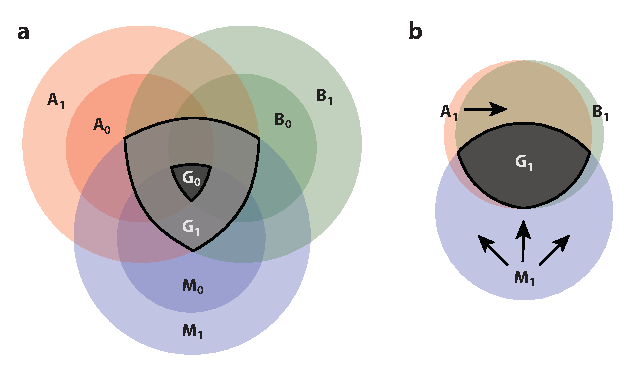
\includegraphics[width=3in]{SampleFigure}
\caption{Figure caption with descriptions of parts a and b}
\label{fig:continuumstuff}
\end{figure}


\begin{textbox}[h]\section{Summary}
TBD  
\end{textbox}


%\subsection{Dynamics}
%turbulence; the dynamical impact of non-ideal MHD terms; accretion flows

%\subsection{Summary}


%Example of a Figure
\section{DEMOGRAPHIC\ INSIGHTS} \label{sec:demographics}
%\subsection{Figures}Figures should be cited in the main text in chronological order. This is dummy text with a citation to the first figure (\textbf{Figure \ref{fig1}}). Citations to \textbf{Figure \ref{fig1}} (and other figures) will be bold. 

\subsection{Links to Host Masses}

\subsection{Environmental Effects}

two key environmental effects, on local scales/``internal" (multiplicity) and global scales/``external" (stripping via tidal encounters or harsh irradiation from nearby massive stars).  

\subsubsection{Multiplicity}
basic mechanics of disk truncation idea.  field population multiplicity rates and separation/eccentricity distributions.  differences there for nearby low-mass clusters.  that implies an expectation that multiplicity is pretty important in shaping observables.  see evidence for diminished continuum luminosities for pairs with closer separations (projected).  weird CB disk exception.  primaries have more mass in majority, but not all, cases.  population of stars in multiples follows similar scaling with host mass.  there is not good evidence for a continuum size vs separation relationship predicted by theory; maybe partly due to not using gas as the tracer, but could also be related to evidence for non-coplanarity (discuss that).  worth noting that fainter disks at smaller separations does not necessarily imply lower densities (consider how much emission you would get for v small optically thick disks).  FIGURE: show separation-Lmm distribution for all available pairs (maybe in left panel of 2-panel figure).

\subsubsection{Close Encounters}
need to read up

\subsubsection{External Photoevaporation}
need to catch up.  FIGURE: probably second panel here showing Lmm versus distance from theta1 Oric.



\subsection{Evolutionary Signatures}

\subsection{Summary}


\section{THE\ EVOLUTION\ OF\ DISK\ SOLIDS} \label{sec:solids}

%The standard assumption is that solids contribute a small fraction, $\sim$1\%, of the total mass budget in a disk.  Even in that case, solids play outsized roles in disks by helping to regulate their thermal balance (as the dominant opacity source) and facilitating complex chemical networks (as the sites of ice-modulated reactions), among other things.  Perhaps most significantly, disk solids are ultimately the seeds for the formation of planets.  As points of reference, the current census of exoplanets indicates that ``rocky" worlds are especially common \citep[e.g.,][]{howard10,dressing13,malhotra15}, and {\it in situ} measurements indicate that the giant planets in our Solar System contain massive sold cores \citep{saumon04,bolton17}.  Constraints on the spatial distribution of solids are essential for developing models of disk physics, and would be crucial resources for understanding the first steps of the planet formation process. 

\subsection{Particle Growth and Migration}

\subsection{Observational Constraints and Conundrums}

% polarization: albedo limits sizes of mm scatterers to ~100um


\subsection{Summary}



\section{SUBSTRUCTURES} \label{sec:substructures}

\subsection{Impact of Pressure Modulations}

\subsection{Potential Origins}

\subsection{``Transition" Disks}

\subsection{``Normal" Disks}

\subsection{Summary}


\section{SYNOPSIS} \label{sec:summary}

%commentary on ``missing mass" arguments (najita/kenyon, greaves, manara).


\section{FUTURE\ PROSPECTS} \label{sec:future}




\begin{figure}[h]
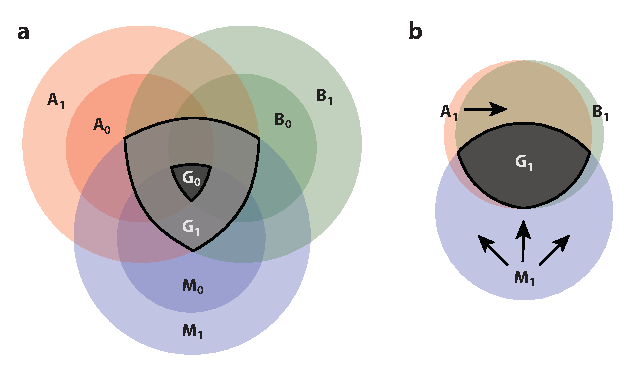
\includegraphics[width=3in]{SampleFigure}
\caption{Figure caption with descriptions of parts a and b}
\label{fig1}
\end{figure}

% Example of a Table
%\subsection{Tables} Tables should also be cited in the main text in chronological order (\textbf {Table \ref{tab1}}).

\begin{table}[h]
\tabcolsep7.5pt
\caption{Table caption}
\label{tab1}
\begin{center}
\begin{tabular}{@{}l|c|c|c|c@{}}
\hline
Head 1 &&&&Head 5\\
{(}units)$^{\rm a}$ &Head 2 &Head 3 &Head 4 &{(}units)\\
\hline
Column 1 &Column 2 &Column3$^{\rm b}$ &Column4 &Column\\
Column 1 &Column 2 &Column3 &Column4 &Column\\
Column 1 &Column 2 &Column3 &Column4 &Column\\
Column 1 &Column 2 &Column3 &Column4 &Column\\
\hline
\end{tabular}
\end{center}
\begin{tabnote}
$^{\rm a}$Table footnote; $^{\rm b}$second table footnote.
\end{tabnote}
\end{table}

% Example of lists
%\subsection{Lists and Extracts} Here is an example of a numbered list:
\begin{enumerate}
\item List entry number 1,
\item List entry number 2,
\item List entry number 3,\item List entry number 4, and
\item List entry number 5.
\end{enumerate}

Here is an example of a extract.
\begin{extract}
This is an example text of quote or extract.
This is an example text of quote or extract.
\end{extract}

%\subsection{Sidebars and Margin Notes}
% Margin Note
\begin{marginnote}[]
\entry{Term A}{definition}
\entry{Term B}{definition}
\entry{Term C}{defintion}
\end{marginnote}

\begin{textbox}[h]\section{SIDEBARS}
Sidebar text goes here.
\subsection{Sidebar Second-Level Heading}
More text goes here.\subsubsection{Sidebar third-level heading}
Text goes here.\end{textbox}



%\subsection{Equations}
% Example of a single-line equation
\begin{equation}
a = b \ {\rm ((Single\ Equation\ Numbered))}
\end{equation}
%Example of multiple-line equation
Equations can also be multiple lines as shown in Equations 2 and 3.
\begin{eqnarray}
c = 0 \ {\rm ((Multiple\  Lines, \ Numbered))}\\
ac = 0 \ {\rm ((Multiple \ Lines, \ Numbered))}
\end{eqnarray}

% Summary Points
\begin{summary}[SUMMARY POINTS]
\begin{enumerate}
\item Summary point 1. These should be full sentences.
\item Summary point 2. These should be full sentences.
\item Summary point 3. These should be full sentences.
\item Summary point 4. These should be full sentences.
\end{enumerate}
\end{summary}

% Future Issues
\begin{issues}[FUTURE ISSUES]
\begin{enumerate}
\item Future issue 1. These should be full sentences.
\item Future issue 2. These should be full sentences.
\item Future issue 3. These should be full sentences.
\item Future issue 4. These should be full sentences.
\end{enumerate}
\end{issues}

%Disclosure
\section*{DISCLOSURE STATEMENT}
If the authors have noting to disclose, the following statement will be used: The authors are not aware of any affiliations, memberships, funding, or financial holdings that
might be perceived as affecting the objectivity of this review. 

% Acknowledgements
\section*{ACKNOWLEDGMENTS}
Acknowledgements, general annotations, funding.

% References
%
% Margin notes within bibliography
\section*{LITERATURE\ CITED}

%To download the appropriate bibliography style file, please see \url{http://www.annualreviews.org/page/authors/author-instructions/preparing/latex}. \\

\noindent
Please see the Style Guide document for instructions on preparing your Literature Cited.

The citations should be listed in alphabetical order, with no titles. For example:






\begin{verbatim}
\begin{thebibliography}{00}

\bibitem[Acevedo \& Fitzjarrald(2001)]{Acevedo:01}
Acevedo O, Fitzjarrald D. 2001.
\textit{J. Atmos. Sci.} 58:2650--67

\bibitem[Acevedo et~al.(2009)Acevedo, Moraes, Degrazia, Fitzjarrald, Manzi \&
  Campos]{Acevedo:09}
\textit{Agric. For. Meteorol.} 149:1--10

\bibitem[Baas et~al.(2006)Baas, Steeneveld, {van de Weil} \& Holtslag]{Baas:09}
Baas P, Steeneveld G, {van de Weil} B, Holtslag A. 2006.
\textit{J. Atmos. Sci.} 63:3045--54

\bibitem[Badran et~al.(1991)]{Badran:91}
Badran F, Thiria S, Crepon M. 1991.
\textit{J. Geophys. Res.} 96:20,521--29

\bibitem[Bakas \& Ioannou(2007)]{Bakas:07}
Bakas NA, Ioannou PJ. 2007.
\textit{J. Atmos. Sci.} 64:1509--29

\bibitem[Calanca et~al.(1998)]{Calanca:98}
Calanca P, Forrer J, Rotach M. 1998.
\textit{Q. J. R. Meteorol. Soc.} 124:1--18

\bibitem[D'Asaro \& Lien(2000)]{DAsaro:00}
D'Asaro EA, Lien RC. 2000.
\textit{J. Phys. Oceanog.} 30:123--45

\bibitem[de~Silva et~al.(1996)de~Silva, Fernando, Eaton \& Hebert]{deSilva:96}
de~Silva I, Fernando H, Eaton F, Hebert D. 1996.
\textit{Earth Planetary Sci. Let.} 143:217--31



\end{thebibliography}
\end{verbatim}


\bibliography{references}


%\begin{thebibliography}{00}

%\bibitem[Alibert et al.(2005)]{alibert05}
%Alibert Y., Mordasini C., Benz W., Winisdoerffer C. 2004.
%\textit{A\&A} 434:343--353

%\bibitem[Cassen \& Moosman(1981)]{cassen81}
%Cassen P., Moosman A. 1981.
%\textit{Icarus} 48:353--376

%\bibitem[Ida \& Lin(2004)]{ida04}
%Ida S., Lin D.N.C. 2004.
%\textit{ApJ} 604:388--413

%\bibitem[Terebey et al.(1984)]{terebey84}
%Terebey S., Shu F.H., Cassen P. 1984.
%\textit{ApJ} 286:529--551

%\end{thebibliography}

%\bibliography{references}

\end{document}
